\chapter{Additional results}
This section contains the detailed studies on the expected results before the unblinding.
The goal of these studies is twofold, as they allow to gauge the expected performance
of the strategies, and to ensure the stability of the analysis by allowing a more in-depth investigation
on the uncertainties and their effect on the signal.

\section{Four lepton channel}
\label{sec:expected_4L}
The likelihood scans and the study on the impact of the systematic uncertainties for each of the strategies
in the four lepton channel are collected here.
First, the studies in the inclusive region are reported in Section~\ref{sec:expected_4L_inclusive}.
Then, the investigations for the triboson fiducial region are detailed in Section~\ref{sec:expected_4L_FSRcut}.

\subsection{Inclusive region}
\label{sec:expected_4L_inclusive}

\subsubsection{Likelihood scans}
% Likelihood scans with nuisance groups without the FSR cut
\label{sec:likelihood_scans_inclusive}
The extraction of the signal strength modifier $\mu$ proceeds through the maximisation of the likelihood,
as described in Section~\ref{sec:statistical_analysis}.
This procedure can be visualised by scanning the likelihood function for several values of the parameter $\mu$ while profiling the nuisance parameters.
For each value the best fit value of the nuisance parameters is computed,
and the resulting value of the likelihood is stored.
These points are then plotted as a function of $\mu$.

Usually the auxiliary quantity $-2\Delta\text{ln}\Likelihood$ (defined as $t_0$ in Equation~\ref{eq:test_statistic})
is used instead of the likelihood itself.
The width of the its profile is linked to the uncertainty on the estimate of $\mu$ from the fit.
More precisely, the set of values $\{ \mu / -2\Delta\text{ln}\Likelihood(\mu) < 1 (4) \}$ corresponds to the 68\usep\% (95\usep\%) confidence interval.

This procedure can also be performed by fixing the values of one or more nuisances instead of allowing them to be fitted by the algorithm.
The effect of fixing the value of one or more parameters is a reduction in the width of the likelihood shape.
This difference is ascribed to the effect of the frozen parameters.

Four groups of parameters are used in the following results:
\begin{itemize}
\item \textbf{theory:} uncertainties on the QCD scale, proton PDFs and on the value of \alpS;
\item \textbf{data-driven:} uncertainties related to the data-driven estimate of fake lepton or fake photon backgrounds;
\item \textbf{luminosity:} the uncertainty on the integrated luminosity corresponding to the data collected by the CMS experiment;
\item \textbf{others:} remaining experimental uncertainties, such as the lepton or photon efficiency scale factors or the \pileup weight;
\end{itemize}

\begin{figure}
  \centering
  \includegraphics[height=.33\textheight]{Figures/dataMC/Run2/phoCR/SR4P/SYS_mZZGloose_central_pow_\dataMCblind .pdf}
  \hfill
  \includegraphics[height=.33\textheight]{Figures/combine/inclusive/scan_\expobs_Run2_SR4P_phoCR_lepCR_mZZGloose.pdf}
  \caption{\captionScan{mass of the $\PZ\PZ\PGg$ system}{Loose}{cut-based ID}{d}{not }}
  \label{fig:scan_Run2_SR4P_phoCR_lepCR_mZZGloose}
\end{figure}

\begin{figure}
  \centering
  \includegraphics[height=.33\textheight]{Figures/dataMC/Run2/lepCR/SR4P/SYS_loosept_central_pow_\dataMCblind .pdf}
  \hfill
  \includegraphics[height=.33\textheight]{Figures/combine/inclusive/scan_\expobs_Run2_SR4P_phoMC_lepCR_mZZGloose.pdf}
  \caption{\captionScan{mass of the $\PZ\PZ\PGg$ system}{Loose}{cut-based ID}{s}{not }}
  \label{fig:scan_Run2_SR4P_phoMC_lepCR_mZZGloose}
\end{figure}

\begin{figure}
  \centering
  \includegraphics[height=0.33\textheight]{Figures/dataMC/Run2/lepCR/SR4P/SYS_mZZGwp90_central_pow_\dataMCblind .pdf}
  \hfill
  \includegraphics[height=.33\textheight]{Figures/combine/inclusive/scan_\expobs_Run2_SR4P_phoMC_lepCR_mZZGwp90.pdf}
  \caption{\captionScan{mass of the $\PZ\PZ\PGg$ system}{\texttt{wp90}}{MVA ID}{s}{not }}
  \label{fig:scan_Run2_SR4P_phoMC_lepCR_mZZGwp90}
\end{figure}

\begin{figure}
  \includegraphics[height=0.33\textheight]{Figures/dataMC/Run2/lepCR/SR4P/SYS_mZZGwp80_central_pow_\dataMCblind .pdf}
  \hfill
  \centering
  \includegraphics[height=.33\textheight]{Figures/combine/inclusive/scan_\expobs_Run2_SR4P_phoMC_lepCR_mZZGwp80.pdf}
  \caption{\captionScan{mass of the $\PZ\PZ\PGg$ system}{\texttt{wp80}}{MVA ID}{s}{not }}
  \label{fig:scan_Run2_SR4P_phoMC_lepCR_mZZGwp80}
\end{figure}

\begin{figure}
  \centering
  \includegraphics[height=.33\textheight]{Figures/dataMC/Run2/lepCR/SR4P/SYS_wp90pt_central_pow_\dataMCblind .pdf}
  \hfill
  \includegraphics[height=.33\textheight]{Figures/combine/inclusive/scan_\expobs_Run2_SR4P_phoMC_lepCR_wp90pt.pdf}
  \caption{\captionScan{transverse momentum of the photon}{\texttt{wp90}}{MVA ID}{s}{not }}
  \label{fig:scan_Run2_SR4P_phoMC_lepCR_wp90pt}
\end{figure}

\begin{figure}
  \centering
  \includegraphics[height=.33\textheight]{Figures/dataMC/Run2/lepCR/SR4P/SYS_MVAcut_central_pow_\dataMCblind .pdf}
  \hfill
  \includegraphics[height=.33\textheight]{Figures/combine/inclusive/scan_\expobs_Run2_SR4P_phoMC_lepCR_MVAcut.pdf}
  \caption{Likelihood scan for the signal strength parameter
    on the yield in the various bins of the photon MVA ID.
    \descriptionFakePhoton{s}.
    The FSR cut is not applied.
    The effect of groups of nuisance parameters on the uncertainty is assessed by sequentially fixing their value in the fit.
  }
  \label{fig:scan_Run2_SR4P_phoMC_lepCR_MVAcut}
\end{figure}

The uncertainty on the signal strength due to the statistics is between 0.35 and 0.50,
and is by far the largest contribution to the total.
This feature is observed for all of the strategies tested here.
The other groups of systematics have much lower impacts.
The theoretical uncertainties are around 0.03-0.05,
while the effect of the luminosity is around 0.03
and the rest of the experimental uncertainties amount to 0.06-0.08 of the signal strength.
The data-driven estimate, when split of the other experimental uncertainties,
adds an undertainty of 0.05-0.08 on the signal strength when estimating the fake photon background
with the data-driven method (Figure~\ref{fig:scan_Run2_SR4P_phoCR_lepCR_mZZGloose}).

\note{Temp}
The signal sample has a cross section of 22.02\usep{}fb, as reported in Table~\ref{tab:listofsamples}.
Assuming a signal strength of
$1.000^{+0.480}_{-0.406}$,
as extracted from
\todo{best strategy}, % TEMP MVAcut
the measured cross section for the production of $\Pp\Pp \to 4\Pl\PGg$ ($\Pl = \Pe,\,\PGm$) at a centre-of-mass energy of $13\TeV$ is
$22.02^{+10.57}_{-8.94}\usep\text{fb}$.


\subsubsection{Systematic impacts}
\label{sec:impacts_inclusive}
\providecommand{\impactswidthscale}{0.6}
The \nonprompt photon contribution is estimated using the data-driven approach.
The variable considered is $m_{\PZ\PZ\PGg}$.
The impacts of the systematic uncertainties on the expected results is shown in Figure \ref{fig:inclusive_cutID_phoCR_mZZGloose}.

\begin{figure}
  \centering
  \includegraphics[height=0.33\textheight]{Figures/dataMC/Run2/phoCR/SR4P/SYS_mZZGloose_central_pow.pdf}
  \hfill
  \includegraphics[height=0.33\textheight]{Run2_SR4P_phoCR_lepCR_mZZGloose_impacts.pdf}
  \caption{Distribution and impacts of the systematic uncertainties on the signal strength fit
    on the mass of the $\PZ\PZ\PGg$ system,
    using the Loose working point of the photon cut-based ID.
    The data-driven estimate for \nonprompt photons is used.
    The FSR cut is not applied.
  }
  \label{fig:inclusive_cutID_phoCR_mZZGloose}
\end{figure}

\begin{figure}
  \centering
  \includegraphics[height=0.33\textheight]{Figures/dataMC/Run2/lepCR/SR4P/lead_loose_pt_pow.pdf}
  \hfill
  \includegraphics[height=0.33\textheight]{Run2_SR4P_phoMC_lepCR_loosept_impacts.pdf}
  \caption{Distribution and impacts of the systematic uncertainties on the signal strength fit
    on the transverse momentum of the photon,
    using the Loose working point of the photon cut-based ID.
    \Nonprompt photons are estimated from simulation.
    The FSR cut is not applied.
  }
  \label{fig:inclusive_cutID_phoMC_loosept}
\end{figure}

\begin{figure}
  \centering
  \includegraphics[height=0.33\textheight]{Figures/dataMC/Run2/lepCR/SR4P/SYS_wp90pt_central_pow.pdf}
  \hfill
  \includegraphics[height=0.33\textheight]{Run2_SR4P_phoMC_lepCR_mZZGwp90_impacts.pdf}
  \caption{Distribution and impacts of the systematic uncertainties on the signal strength fit
    on the mass of the $\PZ\PZ\PGg$ system,
    using the \texttt{wp90} working point of the photon MVA ID.
    \Nonprompt photons are estimated from simulation.
    The FSR cut is not applied.
  }
  \label{fig:inclusive_mvaID_phoMC_mZZGwp90}
\end{figure}

\begin{figure}
  \centering
  \includegraphics[height=0.33\textheight]{Figures/dataMC/Run2/lepCR/SR4P/SYS_wp80pt_central_pow.pdf}
  \hfill
  \includegraphics[height=0.33\textheight]{Run2_SR4P_phoMC_lepCR_mZZGwp80_impacts.pdf}
  \caption{Distribution and impacts of the systematic uncertainties on the signal strength fit
    on the mass of the $\PZ\PZ\PGg$ system,
    using the \texttt{wp80} working point of the photon MVA ID.
    \Nonprompt photons are estimated from simulation.
    The FSR cut is not applied.
  }
  \label{fig:inclusive_mvaID_phoMC_mZZGwp80}
\end{figure}

\begin{figure}
  \centering
  \includegraphics[height=0.33\textheight]{Figures/dataMC/Run2/lepCR/SR4P/SYS_MVAcut_central_pow.pdf}
  \hfill
  \includegraphics[height=0.33\textheight]{Run2_SR4P_phoMC_lepCR_MVAcut_impacts.pdf}
  \caption{Distribution and impacts of the systematic uncertainties on the signal strength fit
    on the yield in the various bins of the photon MVA ID.
    \Nonprompt photons are estimated from simulation.
    The FSR cut is not applied.
  }
  \label{fig:inclusive_kin_phoMC_MVAcut}
\end{figure}


\subsection{Triboson fiducial region}
\label{sec:expected_4L_FSRcut}
The following results are derived after the application of the cut
designed to suppress FSR and enhance the fraction of events from triboson production diagrams,
described in Section~\ref{sec:FSR_cut}.
The target is the process $\Pp\Pp \to \PZ\PZ\PGg \to 4\Pl\PGg$.

\subsubsection{Likelihood scans}
\label{sec:likelihood_scans_FSRcut}

\begin{figure}
  \centering
  \includegraphics[height=.33\textheight]{Figures/dataMC_FSRcut/Run2/phoCR/SR4P/SYS_mZZGloose_central_pow\dataMCblind .pdf}
  \hfill
  \includegraphics[height=.33\textheight]{Figures/combine/FSRcut/scan_\expobs_Run2_SR4P_phoCR_lepCR_mZZGloose.pdf}
  \caption{\captionScan{mass of the $\PZ\PZ\PGg$ system}{Loose}{cut-based ID}{d}{}}
  \label{fig:scan_FSRcut_Run2_SR4P_phoCR_lepCR_mZZGloose}
\end{figure}

\begin{figure}
  \centering
  \includegraphics[height=.33\textheight]{Figures/dataMC_FSRcut/Run2/lepCR/SR4P/SYS_mZZGloose_central_pow\dataMCblind .pdf}
  \hfill
  \includegraphics[height=.33\textheight]{Figures/combine/FSRcut/scan_\expobs_Run2_SR4P_phoMC_lepCR_mZZGloose.pdf}
  \caption{\captionScan{mass of the $\PZ\PZ\PGg$ system}{Loose}{cut-based ID}{s}{}}
  \label{fig:scan_FSRcut_Run2_SR4P_phoMC_lepCR_mZZGloose}
\end{figure}

\begin{figure}
  \centering
  \includegraphics[height=.33\textheight]{Figures/dataMC_FSRcut/Run2/lepCR/SR4P/SYS_loosept_central_pow\dataMCblind .pdf}
  \hfill
  \includegraphics[height=.33\textheight]{Figures/combine/FSRcut/scan_\expobs_Run2_SR4P_phoMC_lepCR_loosept.pdf}
  \caption{\captionScan{transverse momentum of the photon}{Loose}{cut-based ID}{s}{}}
  \label{fig:scan_FSRcut_Run2_SR4P_phoMC_lepCR_loosept}
\end{figure}

\begin{figure}
  \centering
  \includegraphics[height=.33\textheight]{Figures/dataMC_FSRcut/Run2/lepCR/SR4P/SYS_mZZGwp90_central_pow\dataMCblind .pdf}
  \hfill
  \includegraphics[height=.33\textheight]{Figures/combine/FSRcut/scan_\expobs_Run2_SR4P_phoMC_lepCR_mZZGwp90.pdf}
  \caption{\captionScan{mass of the $\PZ\PZ\PGg$ system}{\texttt{wp90}}{MVA ID}{s}{}}
  \label{fig:scan_FSRcut_Run2_SR4P_phoMC_lepCR_mZZGwp90}
\end{figure}

\begin{figure}
  \centering
  \includegraphics[height=.33\textheight]{Figures/dataMC_FSRcut/Run2/lepCR/SR4P/SYS_wp90pt_central_pow\dataMCblind .pdf}
  \hfill
  \includegraphics[height=.33\textheight]{Figures/combine/FSRcut/scan_\expobs_Run2_SR4P_phoMC_lepCR_wp90pt.pdf}
  \caption{\captionScan{transverse momentum of the photon}{\texttt{wp90}}{MVA ID}{s}{}}
  \label{fig:scan_FSRcut_Run2_SR4P_phoMC_lepCR_wp90pt}
\end{figure}

\begin{figure}
  \includegraphics[height=.33\textheight]{Figures/dataMC_FSRcut/Run2/lepCR/SR4P/SYS_mZZGwp80_central_pow\dataMCblind .pdf}
  \hfill
  \centering
  \includegraphics[height=.33\textheight]{Figures/combine/FSRcut/scan_\expobs_Run2_SR4P_phoMC_lepCR_mZZGwp80.pdf}
  \caption{\captionScan{mass of the $\PZ\PZ\PGg$ system}{\texttt{wp80}}{MVA ID}{s}{}}
  \label{fig:scan_FSRcut_Run2_SR4P_phoMC_lepCR_mZZGwp80}
\end{figure}

\begin{figure}
  \centering
  \includegraphics[height=.33\textheight]{Figures/dataMC_FSRcut/Run2/lepCR/SR4P/SYS_MVAcut_central_pow\dataMCblind .pdf}
  \hfill
  \includegraphics[height=.33\textheight]{Figures/combine/FSRcut/scan_\expobs_Run2_SR4P_phoMC_lepCR_MVAcut.pdf}
  \caption{Likelihood scan for the signal strength parameter
    on the yield in the various bins of the photon MVA ID.
    \descriptionFakePhoton{s}.
    The FSR cut is applied.
    The effect of groups of nuisance parameters on the uncertainty is assessed by sequentially fixing their value in the fit.
  }
  \label{fig:scan_FSRcut_Run2_SR4P_phoMC_lepCR_MVAcut}
\end{figure}

Similarly to the inclusive selection, the sensitivity is dominated by the statistics,
with a symmetric impact on the signal strength ranging from 0.4 to 0.5.
The second most impacting group are the experimental uncertainties
which range from around $-0.05/+0.08$ to $-0.07/0.10$ depending on the strategy.
Theoretical uncertainties range from 0.03 to 0.05 and tend to have a symmetric effect on the signal uncertainty.
The luminosity has a smallest contribution, around $-0.03/+0.04$ for all of the strategies.
When applied, the uncertainty on the data-driven fake photon background shifts the signal strength by $-0.04/+0.08$.

\begin{table}
  \caption{
    Summary of the likelihood scans for the four lepton channel
    in the triboson fiducial region
    and contribution from each of the nuisance parameter groups to the total uncertainty on the signal strength.
  }
  \label{tab:scanl_SR4P_FSRcut}
  \small
  \resizebox{\textwidth}{!}{
  \begin{tabular}{lccccccccc}
    \toprule
    Fake photon & data-driven    &    MC          &    MC         &    MC          &    MC         &    MC          &    MC         \\
    Fake lepton & data-driven    & data-driven    & data-driven   & data-driven    & data-driven   & data-driven    & data-driven   \\
    Photon ID   & Loose (cut)    & Loose (cut)    & Loose (cut)   & wp90 (MVA)     & wp90 (MVA)    & wp80 (MVA)     & kinematic     \\
    Variable    &$m_{\PZ\PZ\PGg}$&$m_{\PZ\PZ\PGg}$& $\pt^\PGg$    &$m_{\PZ\PZ\PGg}$& $\pt^\PGg$    &$m_{\PZ\PZ\PGg}$& MVAcut        \\
    \midrule
    $\mu$       & 1.000000       & 1.000000       & 1.000000      & 1.000000       & 1.000000      & 1.000000       & 1.000000      \\
    total       & -0.424/+0.513  & -0.425/+0.503  & -0.431/+0.514 & -0.406/+0.480 & -0.414/+0.493  & -0.415/+0.496  & -0.404/+0.476 \\
    \hline
    data-driven & -0.037/+0.078  & -0.001/+0.001  & -0.001/+0.001 & -0.001/+0.001  & -0.001/+0.001 & -0.001/+0.001  & -0.002/+0.002 \\
    luminosity  & -0.026/+0.046  & -0.028/+0.043  & -0.028/+0.043 & -0.027/+0.041  & -0.027/+0.042 & -0.026/+0.040  & -0.031/+0.047 \\
    theory      & -0.030/+0.031  & -0.042/+0.040  & -0.040/+0.038 & -0.037/+0.034  & -0.037/+0.035 & -0.034/+0.031  & -0.050/+0.056 \\
    syst        & -0.043/+0.081  & -0.053/+0.080  & -0.052/+0.080 & -0.050/+0.076  & -0.050/+0.076 & -0.048/+0.072  & -0.065/+0.095 \\
    stat        & -0.419/+0.498  & -0.419/+0.493  & -0.425/+0.504 & -0.400/+0.471  & -0.409/+0.484 & -0.410/+0.488  & -0.394/+0.461 \\
    \bottomrule
  \end{tabular}
  }
\end{table}

Choosing the strategy that estimates the fake leptons from data while the fake photons are taken from simulation,
and identifies the photon with the \texttt{wp90} working point of the MVA-based ID,
the fit to the $m_{4\Pl\PGg}$ results in an expected signal strength of
$1.000{}^{+0.551}_{-0.426}$
($1.000{}^{+0.028}_{-0.015}\lum {}^{+0.014}_{-0.015}\thy {}^{+0.063}_{-0.032}\syst {}^{+0.546}_{-0.424}\stat$).

As discussed in Section~\ref{sec:likelihood_scans_inclusive},
the $\mathcal{B}(4\Pl)\times\sigma$, with $\Pl = \Pe, \PGm$, of the signal sample is 9.787\usep fb.
Furthermore, referring to the generator-level study described in Section~\ref{sec:signal_genstudy},
the 52\usep\% of the events passing the full selection and the cut to suppress the FSR contribution
are actually from triboson production $\Pp\Pp \to \PZ\PZ\PGg$.
Thus the cross section from the simulation is 5.089\usep fb.

The measured cross section for the process $\Pp\Pp \to \PZ\PZ\PGg \to 4\Pl\PGg$,
with $\Pl = \Pe, \PGm$ is
$5.089{}^{+2.804}_{-2.168}$\usep fb
($5.089{}^{+0.142}_{-0.076}\lum {}^{+0.071}_{-0.076}\thy {}^{+0.321}_{-0.163}\syst {}^{+2.779}_{-2.158}\stat$\usep fb)
at a centre-of-mass energy of 13\TeV.

\paragraph{Observed\\}
\begin{figure}
  \renewcommand{\dataMCblind}{}
  \renewcommand{\expobs}{observed}
  \centering
  \includegraphics[height=.33\textheight]{Figures/dataMC/Run2/lepCR/SR4P/SYS_mZZGwp80_central_pow\dataMCblind .pdf}
  \hfill
  \includegraphics[height=.33\textheight]{Figures/combine/inclusive/scan_\expobs_Run2_SR4P_phoMC_lepCR_mZZGwp80.pdf}
  \caption{\captionScan{mass of the $\PZ\PZ\PGg$ system}{\texttt{wp80}}{MVA ID}{s}{not }}
  \label{fig:scan_observed_FSRcut_Run2_SR4P}
\end{figure}

\note{
This is just a placeholder to dump the unblinded results for the triboson fiducial region 4L, which will be inserted in the previous paragraph.}
The strategy is: see the unblinded scan in Figure~\ref{fig:scan_observed_FSRcut_Run2_SR4P} and the impacts in Figure~\ref{fig:impacts_observed_FSRcut_Run2_SR4P}.

The signal strength is $0.775{}^{+0.391}_{-0.301}$
\\
($0.775{}^{+0.019}_{-0.010}\lum {}^{+0.012}_{-0.013}\thy {}^{+0.044}_{-0.024}\syst {}^{+0.388}_{-0.300}\stat$).

The measured cross section is
$3.944{}^{+1.988}_{-1.534}$\usep fb
\\
($3.944{}^{+0.099}_{-0.051}\lum {}^{+0.059}_{-0.067}\thy {}^{+0.225}_{-0.122}\syst {}^{+1.972}_{-1.526}\stat$\usep fb).


\subsubsection{Systematic impacts}
\label{sec:impacts_FSRcut}

\begin{figure}
  \centering
  \includegraphics[height=0.33\textheight]{Figures/dataMC_FSRcut/Run2/phoCR/SR4P/SYS_mZZGloose_central_pow.pdf}
  \hfill
  \includegraphics[height=0.33\textheight]{Figures/combine/noPixVeto-mZ81/Run2_SR4P_phoCR_lepCR_mZZGloose_impacts.pdf}
  \caption{\captionImpact{mass of the $\PZ\PZ\PGg$ system}{Loose}{cut-based ID}{d}{}}
  \label{fig:FSRcut_cutID_phoCR_mZZGloose}
\end{figure}

\begin{figure}
  \centering
  \includegraphics[height=0.33\textheight]{Figures/dataMC_FSRcut/Run2/lepCR/SR4P/lead_loose_pt_pow.pdf}
  \hfill
  \includegraphics[height=0.33\textheight]{Figures/combine/noPixVeto-mZ81/Run2_SR4P_phoMC_lepCR_loosept_impacts.pdf}
  \caption{\captionImpact{transverse momentum of the photon}{Loose}{cut-based ID}{s}{}}
  \label{fig:FSRcut_cutID_phoMC_loosept}
\end{figure}

\begin{figure}
  \centering
  \includegraphics[height=0.33\textheight]{Figures/dataMC_FSRcut/Run2/lepCR/SR4P/SYS_wp90pt_central_pow.pdf}
  \hfill
  \includegraphics[height=0.33\textheight]{Figures/combine/noPixVeto-mZ81/Run2_SR4P_phoMC_lepCR_mZZGwp90_impacts.pdf}
  \caption{\captionImpact{mass of the $\PZ\PZ\PGg$ system}{\texttt{wp90}}{MVA ID}{s}{}}
  \label{fig:FSRcut_mvaID_phoMC_mZZGwp90}
\end{figure}

\begin{figure}
  \centering
  \includegraphics[height=0.33\textheight]{Figures/dataMC_FSRcut/Run2/lepCR/SR4P/SYS_wp80pt_central_pow.pdf}
  \hfill
  \includegraphics[height=0.33\textheight]{Figures/combine/noPixVeto-mZ81/Run2_SR4P_phoMC_lepCR_mZZGwp80_impacts.pdf}
  \caption{\captionImpact{mass of the $\PZ\PZ\PGg$ system}{\texttt{wp80}}{MVA ID}{s}{}}
  \label{fig:FSRcut_mvaID_phoMC_mZZGwp80}
\end{figure}

\begin{figure}
  \centering
  \includegraphics[height=0.33\textheight]{Figures/dataMC_FSRcut/Run2/lepCR/SR4P/SYS_MVAcut_central_pow.pdf}
  \hfill
  \includegraphics[height=0.33\textheight]{Figures/combine/noPixVeto-mZ81/Run2_SR4P_phoMC_lepCR_MVAcut_impacts.pdf}
  \caption{Distribution and impacts of the systematic uncertainties on the signal strength fit
    on the yield in the various bins of the photon MVA ID.
    \descriptionFakePhoton{s}.
    The FSR cut is not applied.
  }
  \label{fig:FSRcut_kin_phoMC_MVAcut}
\end{figure}


\section{Studies on the \nonprompt photon background}
\label{sec:phFRstudies}
The uncertainty on the fake photon background has different sources,
depending on whether it is estimated with simulation or using a data-driven method:
\begin{enumerate}
\item the uncertainty on the value of the fake rate itself,
      mainly due to the amount of data in the measurement region $\PZ+\text{L}$;
\item the uncertainty due to the limited number of events
      in the fake rate application region, especially for the four lepton channel;
\item the different background composition between the measurement and application region;
\item the mismodelling of the simulation of the processes that result in \nonprompt photons
      and their identification by the detector and the reconstruction algorithm.
\end{enumerate}

The first three affect only the data-driven estimate,
while the last is the main uncertainty when using the simulation to estimate the fake photon background.
However, it also impacts the data-driven method, as the prompt photons in the measurement region are subtracted
using the simulation of the $\PZ+\PGg$ process.

%% \note{We should decide which uncertainties are included in the (arbitrary) flat 50\usep\% normalization uncertainty, if any.}

%% The first source is the uncertainty on the fake rate itself, which is measured in data in the $\PZ+\text{L}$ region.
%% The second source is the limited amount of data in the fake rate application region.
%% Another source is the difference in background composition between the fake rate measurement region and the signal region.
%% These affect only the data-driven estimate.

%% When using the simulation of the \nonprompt photon background, the main uncertainty
%% is the modelling accuracy of such process in the various background samples.
%% This uncertainty is difficult to evaluate, and the method used in this analysis to estimate it
%% is to compare the fake rate measured in data to the one calculated in the samples with \nonprompt photons.

\subsection[Uncertainty on the normalization of gg to 4l]{Uncertainty on the normalization of $\Pg\Pg \to 4\Pl$}
\label{gg4l_normgroup}
The normalization uncertainty on the three samples $\Pg\Pg \to 4\Pe$, $\Pg\Pg \to 2\Pe2\PGm$ and $\Pg\Pg \to 4\PGm$
can be applied as a single nuisance parameter common to all of them
or as three separate parameters that are determined separately in the fit.

The difference between the two approaches, which is expected to be really small,
is evaulated by comparing the expected significances, as shown in Table \ref{tab:grupnorm_cross_check_significance}.
As anticipated, the changes are negligible, usually less than or equal to $0.1\usep\sigma$,
except for the last strategy, where the expected significance changes by $\approx 0.2\usep\sigma$.

\begin{table}
  \caption{Expected significance with the various strategies,
    when the uncertainty on the normalization of the $\Pg\Pg \to 4\Pl$ samples is
    grouped into a single parameter or split into three, one for each final state.}
  \label{tab:grupnorm_cross_check_significance}
  \centering
  \begin{tabular}{l l l c c}
    \toprule
    \multicolumn{3}{c}{Strategy} & \multirow{2}{*}{\shortstack{Significance\\(single)}} & \multirow{2}{*}{\shortstack{Significance\\(split)}}\\
    \noalign{\vspace{.1ex}}\cline{1-3}\noalign{\vspace{.1ex}}
    Photon ID & \nonprompt \PGg & Variable\\
    \midrule
    Cut-based Loose  & data-driven & $m_{\PZ\PZ\PGg}$ & 4.54 & 4.54 \\
    Cut-based Loose  & simulation  & $m_{\PZ\PZ\PGg}$ & 4.60 & 4.65 \\
    Cut-based Loose  & simulation  & $\pt^\PGg$       & 4.53 & 4.57 \\
    MVA ({\tt wp90}) & simulation  & $m_{\PZ\PZ\PGg}$ & 5.06 & 5.13 \\
    MVA ({\tt wp90}) & simulation  & $\pt^\PGg$       & 5.00 & 5.07 \\
    MVA ({\tt wp80}) & simulation  & $m_{\PZ\PZ\PGg}$ & 5.20 & 5.30 \\
    Kinematic        & simulation  & MVA score        & 5.34 & 5.55 \\
    \bottomrule
  \end{tabular}
\end{table}


\subsection{Uncertainty on the fake rate}
The photon fake rate is also affected by the amount of data in the measurement region.
Its impact is evaluated by propagating this uncertainty
through the per-event transfer factor (see Equation~\ref{eq:fakeRate_explanation_part2}),
and constructing the systematic variations of the histograms used for the fit.
It results in a decrease of the expected significance of $\approx 0.09\usep\sigma$.

\subsection{Number of events in the application region}
A major contribution to the uncertainty of the data-driven estimate of the fake photon background
is the limited amount of data in the application region, especially in the four lepton channel.
It is modelled with a Gamma function (see Equation~\ref{eq:gammadef}).
The application of this uncertainty reduces the expected significance by $\approx 0.02\usep\sigma$
in the inclusive region of the four lepton channel.

\subsection{Unified fake rate for all data-taking periods}
As stated in Section~\ref{sec:fake_photons_background}, the photon fake rate is derived separately for the four data-taking periods of \Run2.
The alternative approach is to derive a single fake rate with a smaller statistical uncertainty,
at the cost of increasing the correlation between the different periods.
The resulting fake rate is shown in Figure~\ref{fig:phFR_Run2}.

The effect is expected to be small due to the limited impact of the uncertainty on the fake rate,
which is purely due to the amount of data in the measurement region.
Indeed, using an unique fake rate correlated among the data-taking periods
results in an increase of the expected significance with the data-driven approach
of $\approx 0.036\usep\sigma$.

\begin{figure}
  \centering
  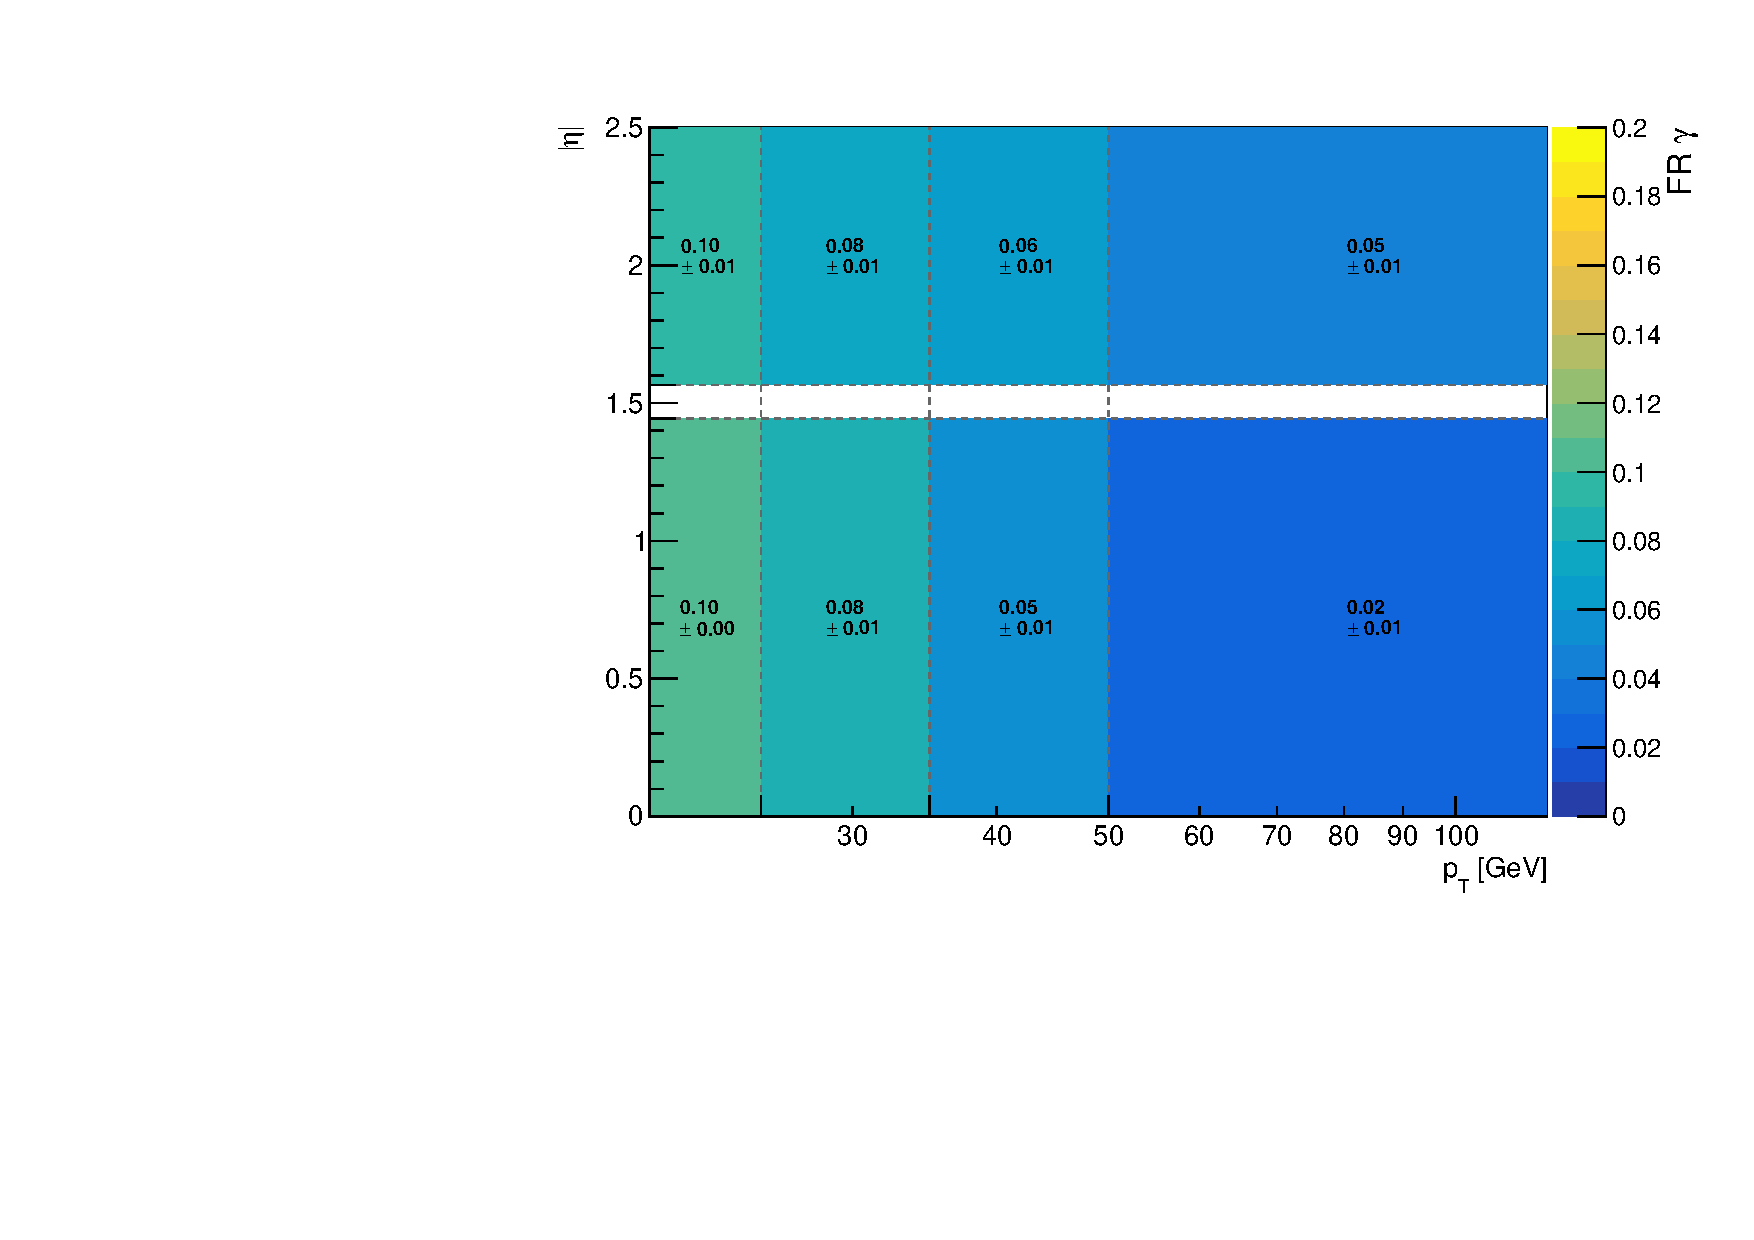
\includegraphics[height=.333333\textheight]{Figures/PhFR/FR_VLtoL_pt-aeta_data-ZGToLLG_Run2.pdf}
  \caption{Photon fake rate measured in the $\PZ+\rm{L}$ region combining events from the four data-taking periods of \Run2.}
  \label{fig:phFR_Run2}
\end{figure}

%% \note{This is the comparison between ``uniqueFR'' and ``ARstat-restorePhFR-groupnorm''.
%% Looking at [control-uniqFR], which is derived using a single FR while leaving the datacard entries \textbf{uncorrelated},
%% suggests that the reduction in the FR uncertainty results in ${+}0.041\usep\sigma$,
%% while the correlation between channels reduces the significance by ${-}0.005\usep\sigma$.}

%% phsigdef                               4.53923  result presented in v1.0
%% restorePhFR-groupnorm-phsigdef         4.45033  (re-)added uncertainty on measured PhFR, stat from CRLFR
%% ARstat-restorePhFR-groupnorm-phsigdef  4.43012  Added gmN representing the stat in the AR (CR4P_1F), uncorrelated between years
%% control-uniqFR                         4.47124  Run with a single FR, derived grouping all events in CRLFR for Run2; do not change the datacard
%% uniqFR                                 4.46641  Make the PhFR correlated, since we used the same values in all the years

